\documentclass[9pt,twocolumn,twoside]{pnas-new}
% Use the lineno option to display guide line numbers if required.
% Note that the use of elements such as single-column equations
% may affect the guide line number alignment.

\usepackage{subcaption}
\usepackage{breqn}
\usepackage{color}

\newcommand\davidsays[1]{{\em\color{blue} {\bf DR:} #1}}

% the follow ing causes latex to not wait interactively
\nonstopmode

\setboolean{displaywatermark}{false}

\templatetype{pnasresearcharticle} % Choose template 
% {pnasresearcharticle} = Template for a two-column research article
% {pnasmathematics} = Template for a one-column mathematics article
% {pnasinvited} = Template for a PNAS invited submission

\title{Brownian dynamics simulation of cytoplasmic dynein's powerstroke reproduces bidirectional stepping}

% Use letters for affiliations, numbers to show equal authorship (if applicable) and to indicate the corresponding author
\author[a,c,1]{Author One}

\affil[a]{Oregon State University}

% Please give the surname of the lead author for the running footer
\leadauthor{Lead author last name} 

% Please include corresponding author, author contribution and author declaration information
\authorcontributions{Please provide details of author contributions here.}
\authordeclaration{Please declare any conflict of interest here.}
\equalauthors{\textsuperscript{1}A.O.(Author One) and A.T. (Author Two) contributed equally to this work (remove if not applicable).}
\correspondingauthor{\textsuperscript{2}To whom correspondence should be addressed. E-mail: author.two\@email.com}

% Keywords are not mandatory, but authors are strongly encouraged to provide them. If provided, please include two to five keywords, separated by the pipe symbol, e.g:
\keywords{dynein $|$ Brownian dynamics $|$ powerstroke $|$ modeling} 

\begin{abstract}
Please provide an abstract of no more than 250 words in a single paragraph. Abstracts should explain to the general reader the major contributions of the article. References in the abstract must be cited in full within the abstract itself and cited in the text.
\end{abstract}

\dates{This manuscript was compiled on \today}
\doi{\url{www.pnas.org/cgi/doi/10.1073/pnas.XXXXXXXXXX}}

\input{../../data/paper_params.tex}

\begin{document}

% Optional adjustment to line up main text (after abstract) of first page with line numbers, when using both lineno and twocolumn options.
% You should only change this length when you've finalised the article contents.
\verticaladjustment{-2pt}

\maketitle
\thispagestyle{firststyle}
\ifthenelse{\boolean{shortarticle}}{\ifthenelse{\boolean{singlecolumn}}{\abscontentformatted}{\abscontent}}{}

%% \dropcap{C}ytoplasmic dynein-1 is a motor protein used to generate directed force in cells. The protein is a homodimer which binds to cellular filaments known as microtubules (MTs). Each monomer has several ATPase domains arranged in a larger globular domain known as the ``head''. This head is the site which hydrolyzes ATP and undergoes the conformational changes responsible for dynein's step. The head is attached via a long chain to the microtubule binding domain (MTBD). Dynein is an interesting structure in that it manages to coordinate ATPase chemistry at its head with MT-releasing chemistry at its MTBD, some 20nm away \cite{mt-atp-coupling}. The head has a long tail domain coming off it, which eventually dimerizes to the other monomer.\\

%% Dynein is unique in that it has a widely varied step size. Dynein's average step is 8 \textit{nm} in the forwards direction, but it is capable of taking 32 \textit{nm} steps in the forwards and reverse directions \cite{weihongpaper} \cite{yildizpaper}. This stochastic, varied stepping is contrasted with the much more regular 8 \textit{nm} step size of kinesin, another bipedal motor protein \cite{kinesin-step-size}. It has been suggested that the long separation between dynein's MTBD and dimerization sites facilitates larger diffusive searches, allowing dynein to take larger steps than kinesin \cite{cargotransport}.\\

%% A simple explanation for dynein's stepping pattern can be given based on only a few facts about the protein. It is known that on treatment with ATP, the tail-head-MTBD angle of a dynein monomer alters, moving the MTBD closer to the tail \cite{carteradpprimed} \cite{burgess-paper}. It is also known that the nucleotide state of the head communicates with the MTBD. ATP binding at a head ATPase shifts the MTBD from a strong to weak MT-bound state. And vice-versa, whether the MTBD is bound or unbound from the MT changes the ATPase rate at the head. From this it is possible to infer a simple model for the dynein stepping cycle. This model, known as the mechanochemical cycle \cite{cianfroccoreview}, has dynein unbind MT, kick forward, diffuse to the next MT binding site, rebind MT, then repeat. Whether a model this simple can explain dynein's behavior needs to be tested.\\

%% Several computational models have been created to explain dynein's motility. \textit{Imamula et. al.} define a chemical transition model which defines all the MT- and nucleotide-bound states dynein goes through as it walks \cite{imamulamodel}. \textit{Sarlah et. al} simulate a model obeying rate constants from \textit{Imamula}, and replicate dynein's stepping trajectory \cite{sarlahmodel}. \textit{Zheng} uses normal mode analysis to simulate the dynein motor's transition from pre to post-powerstroke \cite{normalmodes}. To our knowledge, no computational model exists which takes into account the microscopic dynamics of protein-water interactions to test whether diffusion is enough for dynein motility. Here we show how a simple Brownian dynamics model can be used to test the mechanochemical cycle picture of dynein processivity.\\


%% Dynein has several cofactors which alter its dynamics. For example, the motor's stall force is tripled when exposed to dynactin and Bic2D \cite{yildizdynactin}. This is odd, since the dynactin- and Bic2D-binding site on dynein is on the tail, far from the motor heads.

\dropcap{D}ynein is a motor protein which generates motion for various cellular processes. Cytoplasmic dynein-1, here referred to as ``dynein,'' is a motor which performs cargo transport and aids in nuclear division. The protein consists of a ring structure of six AAA+ domains known as the ``head'' which connect via a long stalk to a microtubule binding domain (MTBD). The AAA+ region is responsible for hydrolyzing ATP to drive dynein's motion. The head is connected via a linker to a large tail domain responsible for binding various cargos and accessory proteins. The tail is also the site of dimerization, where two dynein monomers join to form a homodimeric unit capable of motion.\\

Dynein's mechanism of motion generation is the least understood of all motor proteins. Kinesin and myosin both take periodic, consistent steps of 8nm. In contrast, dynein is known to take highly variant steps both forwards and backwards, but averaging 16nm \cite{yildizpaper, weihongpaper}. Another interesting feature of dynein is the 20nm separation between its ATP hydrolysis and the site and MT binding site \cite{3vkh-cite}. The protein must transmit information about ATP binding across this distance in order to coordinate its steps \cite{mt-atp-coupling}. Explaining these phenomena is necessary to fully understand dynein's mechanism.\\

Studies over the past 15 years have shed much light on dynein's stepping mechanism. The motor is known to switch between two conformational states depending on its ATP hydrolysis state \cite{burgess-paper, FRETstatepaper, carter-paper, nicastro, schmidt-carter}. It is also known that ATP binding can induce structural changes within the motor which increase unbinding rate \cite{leschziner, carter-paper}, and similarly that microtubule rebinding can influence nucleotide unbinding rate \cite{mt-atp-coupling}. Taken together this evidence is synthesized into a powerstroke model \cite{cianfroccoreview, imamulamodel}. In the powerstroke model, dynein binds ATP, causing structural changes which eventually lead to microtubule unbinding at its MTBD. These structural changes transition the motor into a more open position, causing the MTBD to diffuse forwards on the microtubule. This biased search is known as the prestroke. Eventually the MTBD rebinds the microtubule, causing structural changes inducing the ejection of hydrolyzed ADP and transitioning back to the closed position. This causes the motor to lurch forward in a process called the powerstroke. The protein is now ready to re-bind ATP and take another step.\\

Ample evidence exists that dynein engages in an ATP-induced prestroke and MT-binding-induced powerstroke. However, to our knowledge, no work has been done to test whether a structural model of dynein obeying the proposed mechanochemical cycle is sufficient to reproduce experimental stepping data. Existing computational models use chemical rate transitions and assume independence of steps, without simulating the entire mechanochemical cycle \cite{sarlahmodel}. No models have combined structural and kinetic data to simulate a dynein model in a biophysically realistic way. It is necessary to do so to properly test the powerstroke hypothesis. Such a study would determine if the powerstroke mechanism is sufficient to explain dynein's walk, or if further explanation is necessary. Others have theorized that elements such as electrostatic interactions with the microtubule \cite{longrangemt}, tension-gating between the two heads \cite{yildizcleary}, or elasticity of the stalk \cite{burgess-paper} are important for dynein's walk. Such a study would be able to find the minimum criteria for generating dynein's motion.\\

Here we present a course-grained model of cytoplasmic dynein which treats its domains as connected rigid bodies. Chemical transitions and conformational changes consistent with the powerstroke model are accounted for via elastic forces. The dynamics are determined using Brownian dynamics. The model is capable of generating directed motility at rates similar to experiment. Further, we show that the model displays more complex behavior, such as tension gating and force-mediated bidirectionality.\\

\section*{Model}

\begin{figure}[tbhp]
\centering
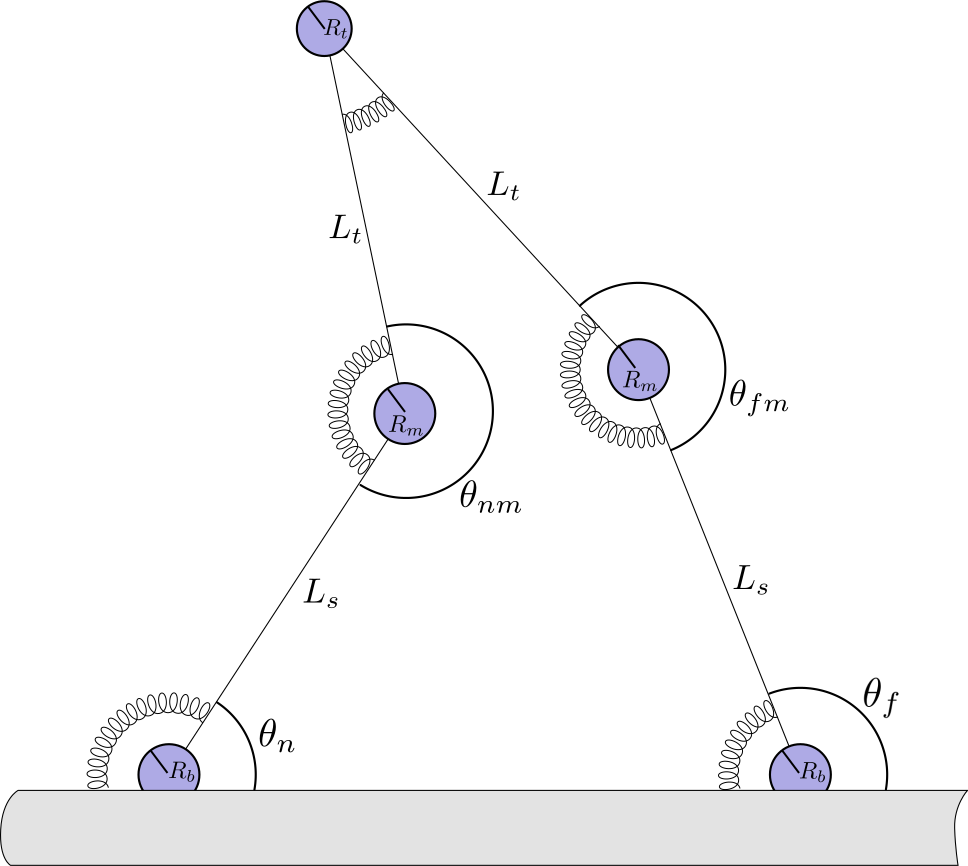
\includegraphics[width=\linewidth]{figures/model-cartoon-simple.pdf}
\caption{TODO: make this more schematic-y and add transition arrows with rates}
\label{fig:model}
\end{figure}

\begin{figure}[tbhp]
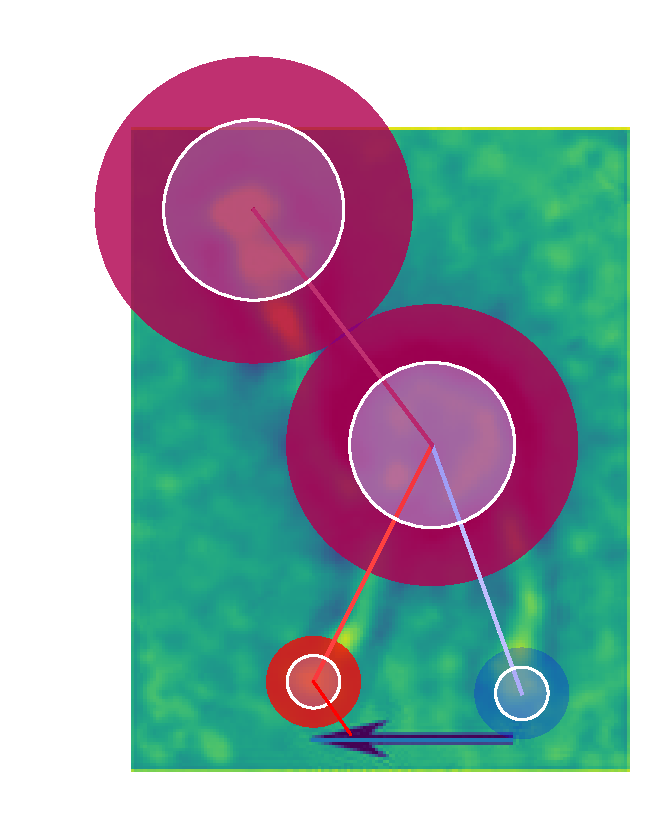
\includegraphics[width=0.4\linewidth]{../../plots/burgess-model-figure.pdf}%
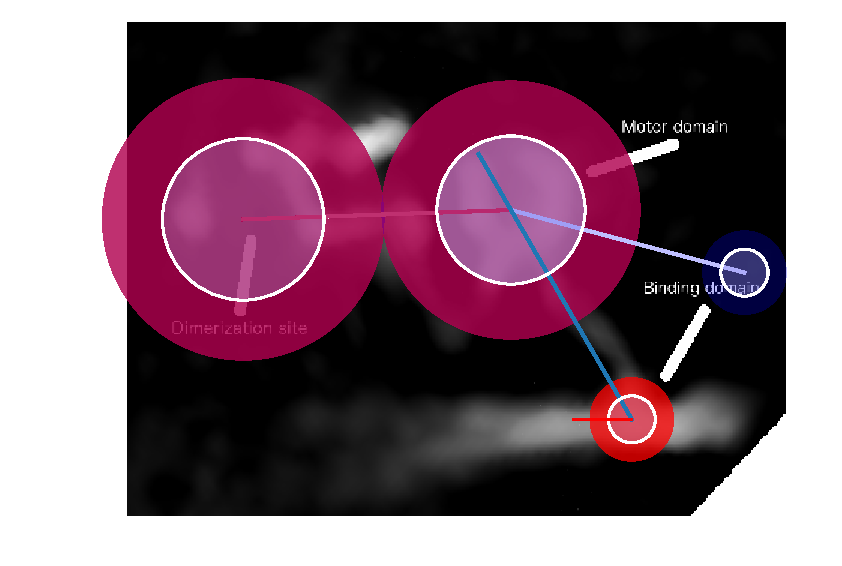
\includegraphics[width=0.6\linewidth]{../../plots/grotjahn-model-figure.pdf}%
%% 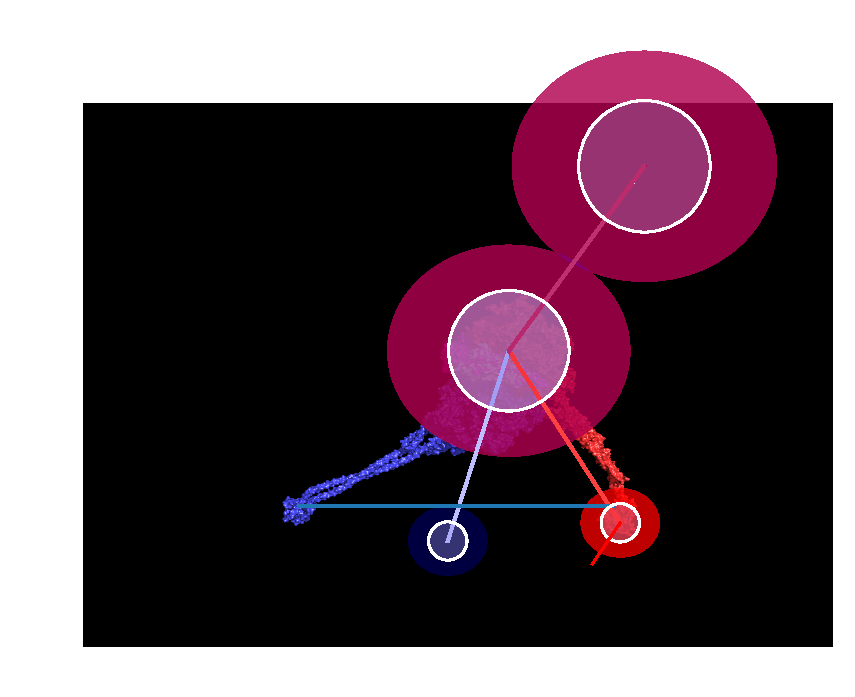
\includegraphics[width=0.3\linewidth]{../../plots/crystal-model-figure.pdf}%
\caption{\textbf{Hinge model compared with dynein micrographs.} \textit{Left:} Model at equilibrium angles superimposed over an axonemal dynein c micrograph consisting of an apo and and ADP-Pi-bound dynein monomer \cite{burgess-paper}; axonemal and cytoplasmic dynein have comparable size and architecture \cite{dynein-c-paper}. \textit{Right:} Model at equilibrium superimposed over full-length dimerized dynein bound to accessory proteins, (map ID EMD-7000) \cite{grotjahn}. Left figure has a scale bar of 15nm, right 26.3nm between MTBD and AAA1 of motor domain.}
\label{fig:micrographs}
\end{figure}

\begin{table}[tbhp]
\centering
\caption{Parameters used in model simulation.}
\label{tab:params}
\begin{tabular}{lrrr}
Parameter & Model & Experimental & Source \\
\midrule
$c_b$ & $\cb \Delta G_{ATP}$ &  & \\
$c_m$ & $\cm \Delta G_{ATP}$ &  & \\
$c_t$ & $\ct \Delta G_{ATP}$ &  & \\
$k_b$ & $\kb s^{-1}$&  & \\
$k_{ub}$ & $\kub s^{-1}$ & & \\
$L_s$ & $\ls nm$ & 21nm & \cite{burgess-paper, 3vkh-cite, carter-paper}\\
$L_t$ & $\lt nm$ & 23nm & \cite{burgess-paper, 3vkh-cite, carter-paper}\\
$c$ & $\cexp$ & & \\
$\theta_b$ & $\eqb$ &  120 & \cite{leschziner} \\
$\theta_m^{\mbox{pre}}$ & $\eqmpre$ &  197 & \cite{burgess-paper}\\
$\theta_m^{\mbox{post}}$ & $\eqmpost$ & 242 & \cite{burgess-paper}\\
$\theta_t$ & $\eqt$ &  & \\
$R_t$ & $\radiust$ & 8nm & \cite{burgess-paper}\\
$R_m$ & $\radiusm$ & 11nm & \cite{burgess-paper}\\
$R_b$ & $\radiusb$ & 3.5nm & \cite{burgess-paper}\\

\bottomrule
\end{tabular}

%% \addtabletext{nomenclature for the TSs refers to the numbered species in the table.}
\end{table}

\section{Model}
This dynein model is meant to capture the coarse-grained structural, dynamical and chemical properties of the full dynein complex while remaining mathematically simple. The structural features of dynein are captured through a two-dimensional geometric model of circular domains connected by rigid rods, shown in Figure \ref{fig:model}. The dynamics of dynein are captured by imposing both equilibrium and Brownian forces on each circular domain of the model. The chemical properties of dynein are captured by sporadically transitioning the model between two states: a ``bothbound'' state where both binding domains are fixed to the microtubule, and a ``onebound'' state where one foot is free to diffuse. Each state feels equilibrium forces meant to mimic the structural changes which occur through dynein's chemical cycle. This transitioning is meant to capture the powerstroke of dynein, between the apo ``post-powerstroke'' state and the ADP-Pi-bound ``pre-powerstroke'' state.

\subsection*{Model geometry}
The dynein model represents a full dynein complex consisting of two dynein heavy chains dimerized by a large tail domain. The model accounts for the following domains within the complex: two microtubule binding domains (``MTBD''), two AAA+ heptad motor domains, and a tail domain consisting of many dynein light chains and a dimerization site. MTBDs, motor domains and the tail are all represented by circles of radius $R_b$, $R_m$ and $R_t$, respectively. Each MTBD is connected to a motor domain via a rigid rod of length $L_s$, meant to represent the stalk domain. Each motor domain is connected to the tail domain via a rigid rod of length $L_t$; this rod represents the heavy chain linker and intermediate/light chains which connect the motor to the dimerization site.\\

Values for $R$ and $L$ were acquired by aligning the dynein model with EM micrographs of the full dynein complex \cite{burgess-paper,grotjahn}, as shown in Figure \ref{fig:micrographs}. See Table \ref{table:params} for these values.\\

\subsection*{Equilibrium forces}
The onebound model has four degrees of freedom: $\theta_{bb}, \theta_{bm}, \theta_{um}$ and $\theta_{ub}$. The bothbound model has two: $\theta_{nm}$ and $\theta_{fm}$. The model is free to vary across all of these degrees of freedom, barring steric interactions with the microtubule. These angles describe a planar model which is not capable of transverse motion. To capture the gross dynamics and interdomain oscillations of the protein, restoring forces are imposed on each angle about equilibrium angles $\theta^{eq}_{bb}, \theta^{eq}_{bm}, \theta^{eq}_{um}, \theta^{eq}_{ub}$ for onebound and $\theta^{eq}_{nm}$ and $\theta^{eq}_{fm}$ for bothbound. Each domain $i$ has a harmonic energy $c_i\left(\theta_i-\theta^{eq}_i\right)^2$ which exerts a restoring force pushing it back to equilibrium, where $c_b$, $c_m$ and $c_t$ are spring constants for each domain. These equilibrium angles are taken to be the average angle occupied by the protein in solution, and are thus extracted from EM micrographs, shown in Figure \ref{fig:micrographs}. Electron microscopy studies using ADP-Vi to freeze dynein in the pre-powerstroke state allow for both pre- and post-stroke equilibrium angles to be found \cite{burgess-paper}.\\

\subsection*{Brownian dynamics}
Brownian dynamics is used to study the model's dynamics in a biophysical manner. In the Brownian regime, protein motion is given by $\dot{\vec{X}} = \frac{1}{\gamma}\left(\vec{F}+\vec{R}\right)$. In the model, each circular domain has its own associated $\gamma$ factor given by Stokes' Law as $\gamma_i = 6\pi\nu R_i$ with dynamic viscosity $\nu$ \cite{stokeslaw}. The force on each domain is given by $\vec{F} = \vec{F}_{spr} + \vec{T}$, where $\vec{T}$ is the tension force between domains maintaining the rigid rod constraint. Each domain feels not only a harmonic restoring force, but also a Brownian force $\vec{R}$. This force is a Gaussian-distributed zero-mean magnitude with variance $R_{\sigma^2} = \sqrt{\frac{2k_bT\gamma}{\delta t}}$ \cite{einstein} and uniformly random direction.

\subsection*{Binding}
Conformational changes on nucleotide binding, also known as the mechanochemical cycle \cite{cianfrocco}, are captured by transitioning the model between the onebound and bothbound states. Binding can occur when the onebound model's unbound foot diffuses near enough the microtubule. When within a distance of $1 A$, binding occurs at a rate of $k_b$ (Table \ref{table:params}). On binding, the onebound model changes state to a bothbound model while retaining the positions of its domains. The previously unbound domain is transported to the microtubule.

\subsection*{Unbinding}
Unbinding occurs when a bothbound MTBD unbinds from the microtubule. This event can occur for either MTBD, and each domain has its own unbinding rate $k_{ub}$. To account for the tension-gating proposed by Yildiz \textit{et al} \cite{yildiz} to allow for interhead communication and bias the motor forward, the parameter $c$ is used to alter the unbinding rates of either MTBD. For domain $i \in \{n, f\}$ with binding domain angle $\theta_{ib}\left(\theta_{nm}, \theta_{fm}\right)$, unbinding rate is given by $k_{ub} = k^0_{ub}e^{-c\left(\theta_{ib}-\theta^{eq}_{ib}\right)}$. This will bias the model to unbind more preferentially for the lagging MTBD due to a higher likelihood for $\theta^{eq}_{ib} > \theta_{ib}$ for the lagging head. Values used for parameters $k^0_{ub}$ and $c$, along with $k_b$, are shown in Table \ref{table:params}.\\

The ``prestroke'' and ``powerstroke'' events in the mechanochemical cycle \cite{cianfrocco} are captured by different motor equilibrium angles between the onebound and bothbound states. The onebound ``prestroke'' state has an unbound motor angle closer to $\pi$ than the bothbound motor\cite{burgess-paper}; thus, on unbinding, the unbound MTBD should experience a restoring force effecting the ``prestroke'' conformational change. On rebinding, the motors transition back to the poststroke equilibrium, producing restoring forces in the direction of the ``powerstroke.''

\matmethods{

  \section*{Fitting $k_b$ and $k_{ub}$}
  To fit the binding and unbinding rate constants $k^0_b$ and $k^0_{ub}$, a simple theoretical model for stepping was used. First, it is assumed that the unbinding rate of an MTBD does not depend on the binding state of the other MTBD. Then the dissociation rate of the whole complex from the microtubule, $k_{dis}$, is estimated as $k_{dis} = P(ob)*k_{ub} = \frac{\bar{t}_{ob}}{\bar{t}_{step}} * \frac{1}{\bar{t}_{bb}}$, where $P(ob)$ is the probability of a dynein complex being in the onebound state, $\bar{t}_{ob}$ and $\bar{t}_{bb}$ are the expected durations for a onebound and bothbound state, and $\bar{t}_{step} = \bar{t}_{ob} + \bar{t}_{bb}$ is the expected step duration. Plugging in the last definition yields $k_{dis} = \frac{\bar{t}_{step} - \bar{t}_{bb}}{\bar{t}_{step}\bar{t}_{bb}}$. Introducing a new variable $\bar{t}_{run}$, the average run length of in vivo dynein, and using the relation $\bar{t}_{run} = k_{dis}^{-1}$, a new relation is found for bothbound time: $\bar{t}_{bb} = \frac{\bar{t}_{run}\bar{t}_{step}}{\bar{t}_{run}+\bar{t}_{step}}$. Using the definition of $\bar{t}_{step}$ a similar relation is found for onebound time: $\bar{t}_{ob} = \frac{\bar{t}_{step}^2}{\bar{t}_{step}+\bar{t}_{run}}$. Finally, using the relation $\bar{t}_{step} = \frac{v}{L_{step}}$ for dynein velocity $v$ and expected tail step length $\bar{L}_{step}$, the following equations are found for onebound and bothbound time in terms of experimental observables of velocity, run time and step length:

  \begin{align}
    \bar{t}_{ob} &= \frac{\bar{L}^2}{\bar{v}^2\left(\bar{L}/v+\bar{t}_{run}\right)}\\
    \bar{t}_{bb} &= \frac{\bar{L}\bar{t}_{run}}{v\left(\bar{t}_{run}+\bar{L}/v\right)}
  \end{align}

  For estimating onebound and bothbound times from Yildiz \textit{et al}\cite{yildiz}, a velocity of $124 nm/s$ is used. A study with a similar velocity is used to estimate $\bar{t}_{run} = 1060 nm / 134 nm / s = 7.9s$ \cite{weihongpaper}. These observables, along with $\bar{L} = 8nm$, yield estimations $\bar{t}_{ob} = 5.2*10^{-4}s$ and $\bar{t}_{bb} = 6.4 * 10^{-2}s$.\\

  \section*{Onebound motion equations derivation}
  Brownian Dynamics was used to describe the motion of each domain, indexing with $i \in \{bb, bm, t, um, ub\}$, corresponding to bound-binding, bound-motor, tail, unbound-motor, unbound-binding:

  \begin{align}
    \dot{X_i} &= \frac{1}{\gamma_i}\left(F^x_i + R^x_i\right)\\
    \dot{Y_i} &= \frac{1}{\gamma_i}\left(F^y_i + R^y_i\right)
  \end{align}

  where $F^{x/y}_i$ is the force projection on coordinate $x/y$ of domain $i$, and $R^x_i$ the Brownian force, a Gaussian zero-mean force with variance $R_{\sigma^2} = \sqrt{\frac{2k_bT\gamma}{\delta t}}$ \cite{einstein}. Transforming position variables to polar coordinates results in four degrees of freedom: $\theta_{bb}, \theta_{bm}, \theta_{um} and \theta_{ub}$. Performing this transformation and expanding the force term yields the following equations:

  \begin{multline}
    \dot{X_i}\left(\theta_{bb}, ..., \theta_{ub}, \dot{\theta}_{bb}, ..., \dot{\theta}_{ub}\right) = \frac{1}{\gamma_i}\big(F^{spr}_x(\theta_{bb}, ..., \theta_{ub}) + \\
    \lambda_i\left(X_{i+1}-X_i\right) + \lambda_{i-1}\left(X_i-X_{i-1}\right)R^x_i\big)
    \label{eq:ob-system}
  \end{multline}

  \begin{multline}
    \dot{Y_i}\left(\theta_{bb}, ..., \theta_{ub}, \dot{\theta}_{bb}, ..., \dot{\theta}_{ub}\right) = \frac{1}{\gamma_i}\big(F^{spr}_y(\theta_{bb}, ..., \theta_{ub}) + \\
    \lambda_i\left(Y_{i+1}-Y_i\right) + \lambda_{i-1}\left(Y_i-Y_{i-1}\right)R^y_i\big)
    \label{eq:ob-system}
  \end{multline}

  where the $\lambda$ terms are tension terms needed to maintain the rigid rod constraints and $\vec{F}^{spr}$ the harmonic equilibrium forces felt by each domain. Each $X_i$ coordinate is related to the $\theta_j$ coordinates via the recursive formulas $X_{i>1} = L_i\cos(\theta_{i-1})+X_{i-1}$ and $Y_{i>1} = L_i\sin(\theta_{i-1})+Y_{i-1}$ for y-coords. Thus, each $\dot{X_i}$ term is linearly related to one or more $\dot{\theta_j}$ terms.\\

  There are $n$ unknown $\theta_j$ values and n unknown $\lambda$ values, totaling $2n$ unknown variables. There are $2n$ equations linear in $\dot{theta_j}$ and $\lambda_q$, $n$ each from the X and Y equations. The system of equations provided by Equation $\ref{eq:ob-system}$ was solved in Matlab, yielding equations for all $\dot{\theta_j}$.

  \section*{Bothbound motion equations derivation}
  Brownian dynamics was also used for the bothbound case. Due to the added constraint of both binding domains being fixed to the microtubule, the model is fully described by angles $\theta_{nm}$ and $\theta_{fm}$; see Figure \ref{fig:model}. The positions of non-bound domains are defined by the following equation for $i \in \{nb, nm, t, fm, fb\}$, corresponding to near-binding, near-motor, tail, far-motor and far-binding domains:

  \begin{multline}
    \dot{X_{i\neq\{nb, fb\}}}\left(\theta_{nm},\theta_{fm}, \dot{\theta_{nm}}, \dot{\theta_{fm}}\right) = \frac{1}{\gamma_i}\big(F^{spr}_x(\theta_{nm}, \theta_{fm}) + \\
    \lambda_i\left(X_{i+1}-X_i\right) + \lambda_{i-1}\left(X_i-X_{i-1}\right) + R^x_i\big)
    \label{eq:bb-system}
  \end{multline}

  \begin{multline}
    \dot{Y_{i\neq\{nb, fb\}}}\left(\theta_{nm},\theta_{fm}, \dot{\theta_{nm}}, \dot{\theta_{fm}}\right) = \frac{1}{\gamma_i}\big(F^{spr}_y(\theta_{nm}, \theta_{fm}) + \\
    \lambda_i\left(Y_{i+1}-Y_i\right) + \lambda_{i-1}\left(Y_i-Y_{i-1}\right) + R^y_i\big)
    \label{eq:bb-system}
  \end{multline}

  Coordinate velocities are similarly linear with $\dot{\theta_{nm}}$ and $\dot{\theta_{fm}}$. This system has six independent equations and six unknowns $\dot{\theta_{nm}}, \dot{\theta_{fm}}, \lambda_{nb}, \lambda_{nm}, \lambda_{t}, \lambda_{fm}$. Analytic solutions were acquired using Mathematica.

  \section*{Simulating the model}
  Simulations began in the bothbound equilibrium state. The model was time-evolved via Euler's Method using analytic expressions for $\{\dot{\theta}_{bb}, \dot{\theta}_{bm}, \dot{\theta}_{um}, \dot{\theta}_{ub}\}$, using a timestep of $dt = 10^{-10}s$. In the onebound state, during each timestep the model had a $k_b*dt$ probability of transitioning into the bothbound state, where $k_b = k_b^0\left(1-H\left(X_{uby}-0.1\right)\right)$, where H is the Heaviside function. On transition to bothbound, proper $\theta_{nm}$ and $\theta_{fm}$ angles and proper interhead separation $L$ were calculated to yield a bothbound model with identical cartesian positions to the old bothbound, except with the previously unbound binding domain moved to $y=0$. Once in bothbound, the model was time-evolved via Euler's Method using analytic expressions for $\{\dot{\theta}_{nm}$ and $\dot{\theta}_{fm}\}$ and a timestep of $dt=10^{-10}s$. Each timestep, the bothbound model had a $k_{ub}*dt$ chance of transitioning to onebound, where $k_{ub} = k^0_{ub}e^{-c(\theta-\theta_{eq})}$. On transitioning, proper values of $\{\theta_{bb}, \theta_{bm}, \theta_{um}, \theta_{ub}\}$ were calculated to create a onebound model with identical cartesian positions to the old bothbound model.\\

  \section*{Calculating leading/lagging probability vs displacement}

  \section*{Calculating force-dependent velocities}
}

\section{Results}

\begin{figure}[tbhp]
\centering
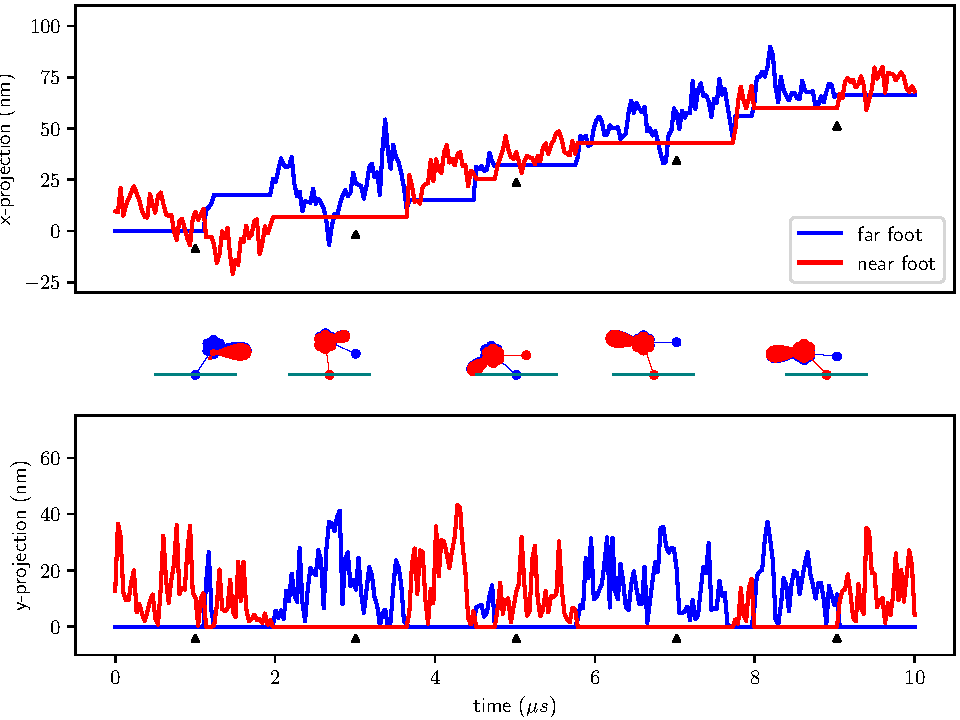
\includegraphics[width=\linewidth]{../../plots/paper_trajectory_plot.pdf}
\caption{\textbf{Model achieves forward-directed processivity.} \textit{Top view:} x-position of near and far binding domains during a 10 $\mu s$ simulation at high kinetic parameters of $k_b = \trajectorykb s^{-1}$ and $k_{ub} = \trajectorykub s^{-1}$. \textit{Middle view:} Cartoon snapshot of model at time indicated by bound binding domain. Teal lines correspond to the microtubule. \textit{Bottom view:} y-projection. Arrows on top and bottom plots correspond to respective snapshot times.}
\label{fig:trajectory}
\end{figure}

\textbf{Processive, forward-directed motility}\\
The model was time-evolved using Euler's method. When simulated, the model produces processive, forward-directed motion. Figure \ref{fig:trajectory} shows a short time window of the model's dynamics. The model is capable of taking both forward and backwards steps, but is biased in the forward direction.\\

\textbf{Stepping dynamics}
The stepping dynamics of the model reproduce experimental results. The model is capable of producing a wide variety of step lengths, from 48nm forward to 40nm backwards, as in Figure \ref{fig:behavior}.a. The onebound and bothbound times correspond well to the theoretical values, as in \ref{fig:behavior}.b and c. The tension-gating mechanism is capable of producing a lagging-head favor, as shown in \ref{fig:behavior}.d.


%% -Briefly how we simulated the model
%% -Model is forwards-directed and processive (trajectory plot)
%% -Tuning the parameters to Yildiz data (kb/kub from theoretical OB/BB time and step length histograms for cm/cb/ct and leading/lagging fractions for c)
%% -Does the tuned model walk similarly to Yildiz dynein? (also the lagging vs step length)

\begin{figure}[tbhp]
  \centering
  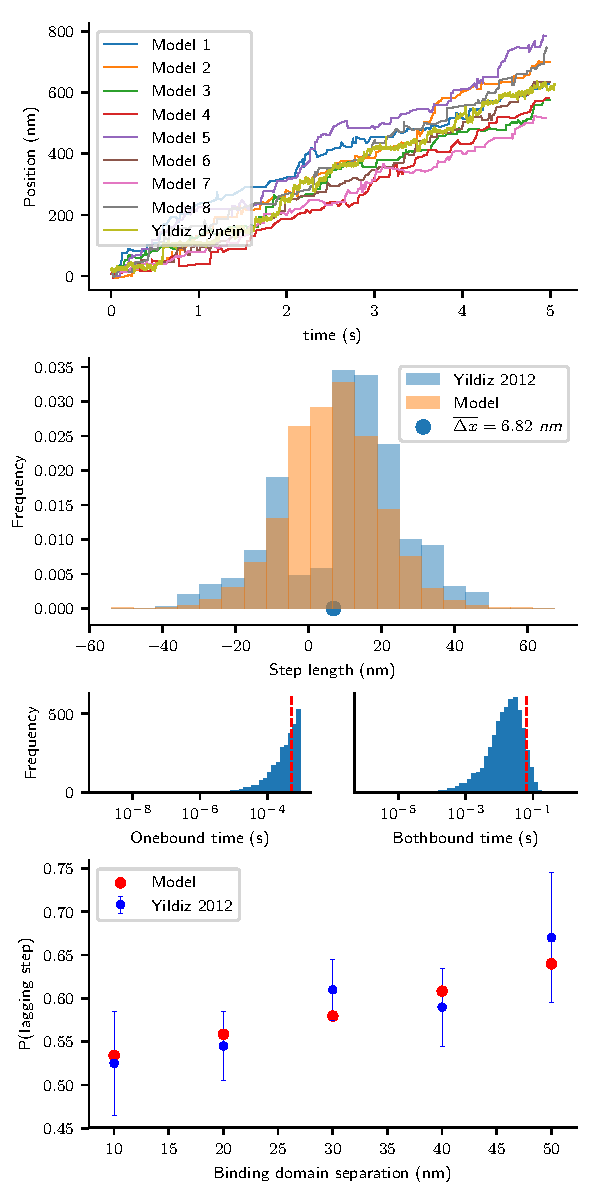
\includegraphics[width=\linewidth]{../../plots/paper_model_behavior}
\caption{\textbf{Basic behavior of our model}}
\label{fig:behavior}
\end{figure}

\begin{figure}[tbhp]
  \centering
  a)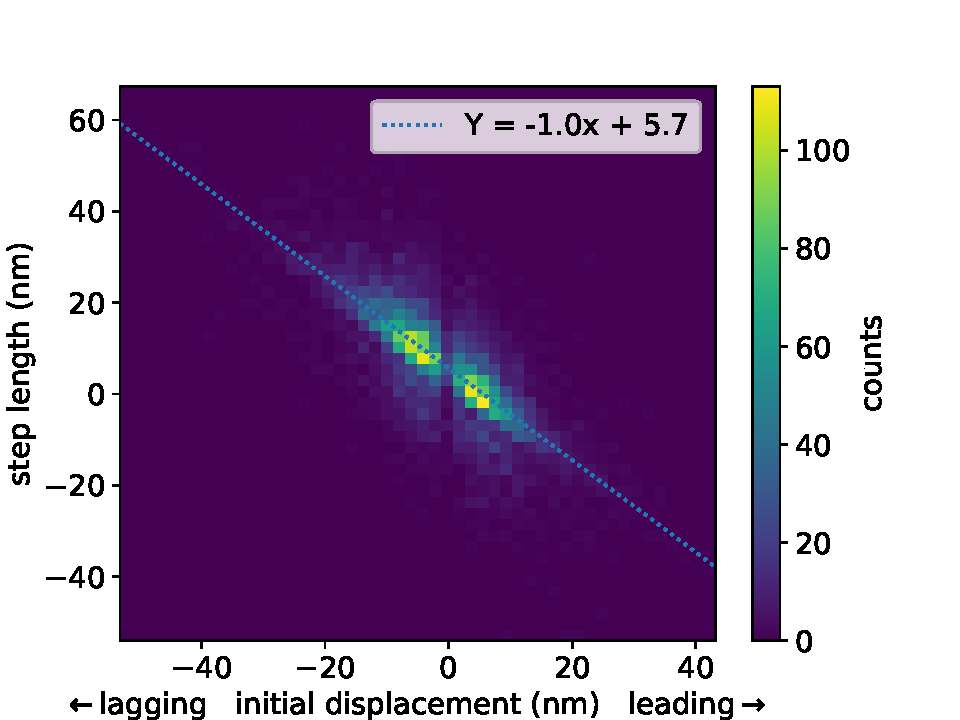
\includegraphics[width=\linewidth]{../../plots/paper_displacement_vs_step_length.pdf}
  b)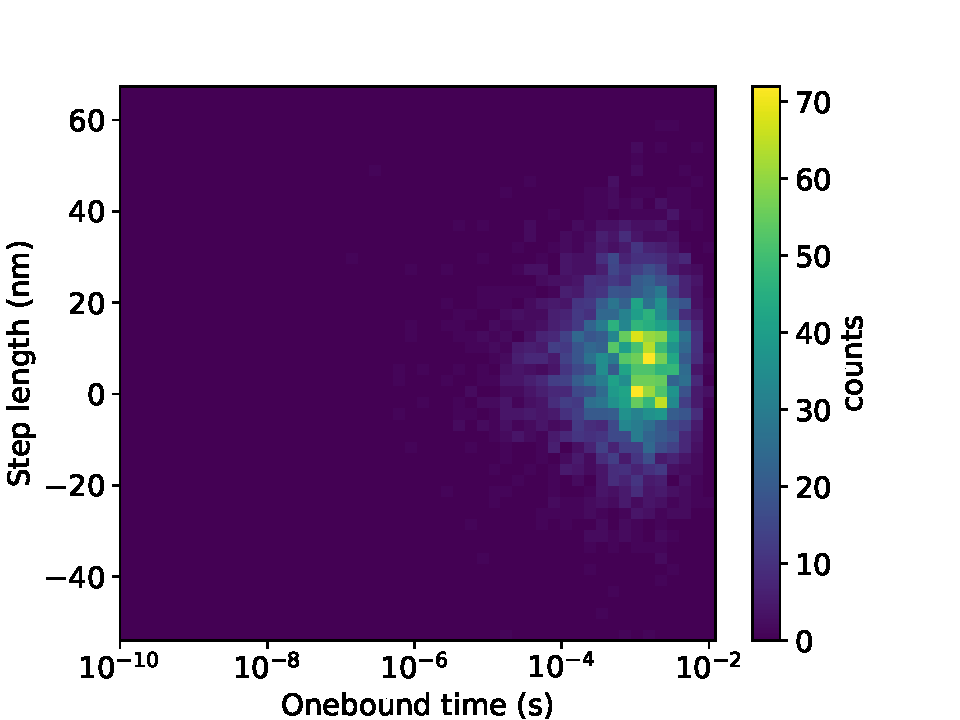
\includegraphics[width=\linewidth]{../../plots/paper_onebound_vs_steplength.pdf}
  c)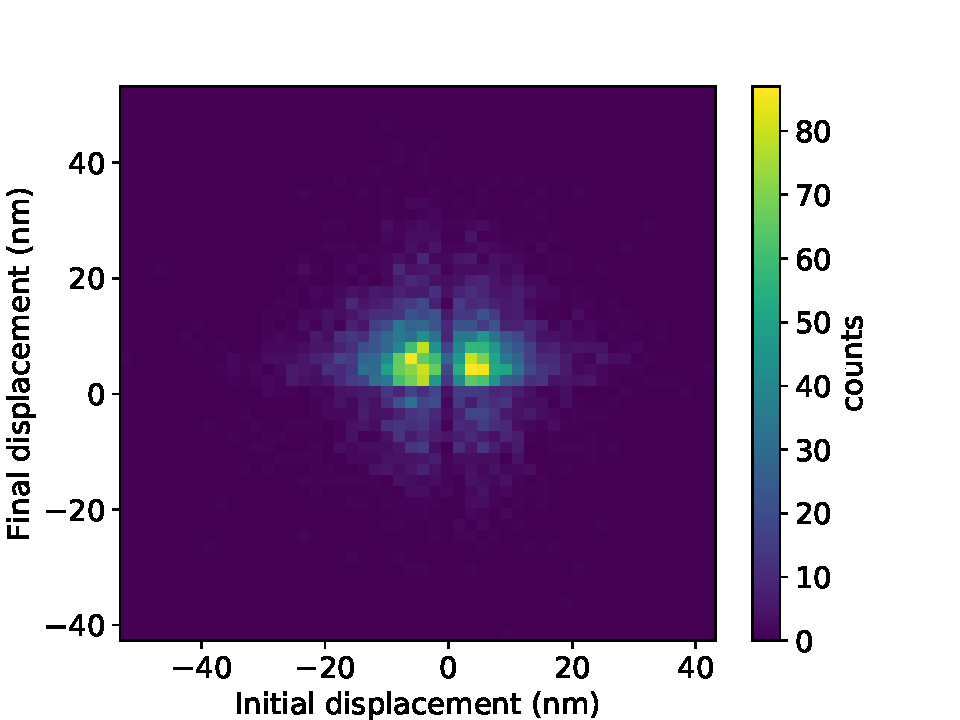
\includegraphics[width=\linewidth]{../../plots/paper_initial_vs_final_displacement.pdf}
  \caption{\davidsays{Look up Yildiz figure for (a)}\textbf{Does our model capture dynamics a markov model wouldn't?}}
\label{fig:}
\end{figure}

\begin{figure}[tbhp]
  \centering
  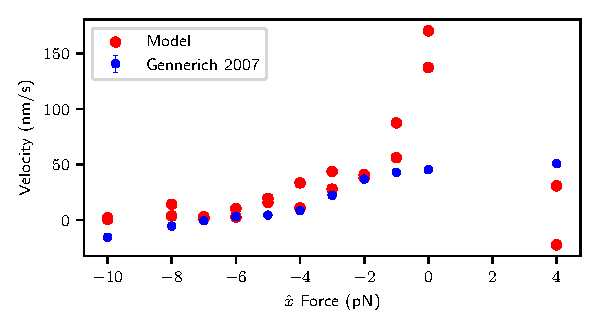
\includegraphics[width=\linewidth]{../../plots/paper_force_vs_velocity.pdf}
\caption{Gennerich et al \cite{responsetoload}}
\label{fig:}
\end{figure}

%% \begin{figure*}[tbhp]
%%     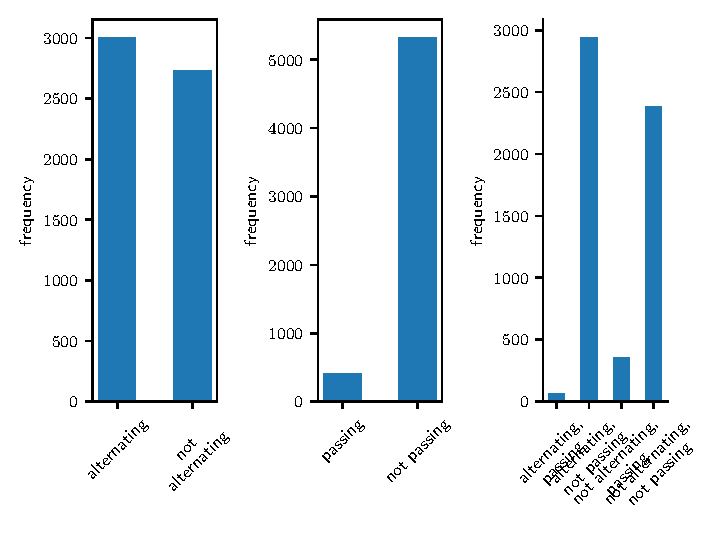
\includegraphics[width=0.5\linewidth]{../../plots/paper_foot_order_histogram.pdf}
%% \caption{The left plot is the $C=0$ case where the unbinding rate is
%%   independent of angle.  Here ``alternating'' means that the binding
%%   domain which did not move last time moved this time.  Passing means
%%   that the moving foot was behind, and ended up in front.}
%% \label{fig:steppingorder}
%% \end{figure*}

\section{Discussion}

\begin{enumerate}
\item \cite{lippert} is a 2017 PNAS paper claiming the powerstroke model is wrong since angular displacement of the dynein ring is weak (+- 7 degrees) and weakly correlated with stepping. However, their camera records at 50ms resolution, which is 100x slower than our average onebound time. Thus their whole experiment is somewhat flawed. This is relevant since the oneboudn time duration may not be well known, and our theoretical results may be relevant.
\item No need for being guided to Mt binding sites, the motor naturally can take 16nm steps through a powerstroke
\item Is tension gating necessary for our model? Could run simulations without it to see how the model changes
\item Dynein's adjacent step step length correlation is low; thus the motor is a memory-less process which could be simulated by a Markov model. Also look at ob and bb time covariance and displacement covariance
\end{enumerate}


%% \begin{figure}[tbhp]
%%   \centering
%%    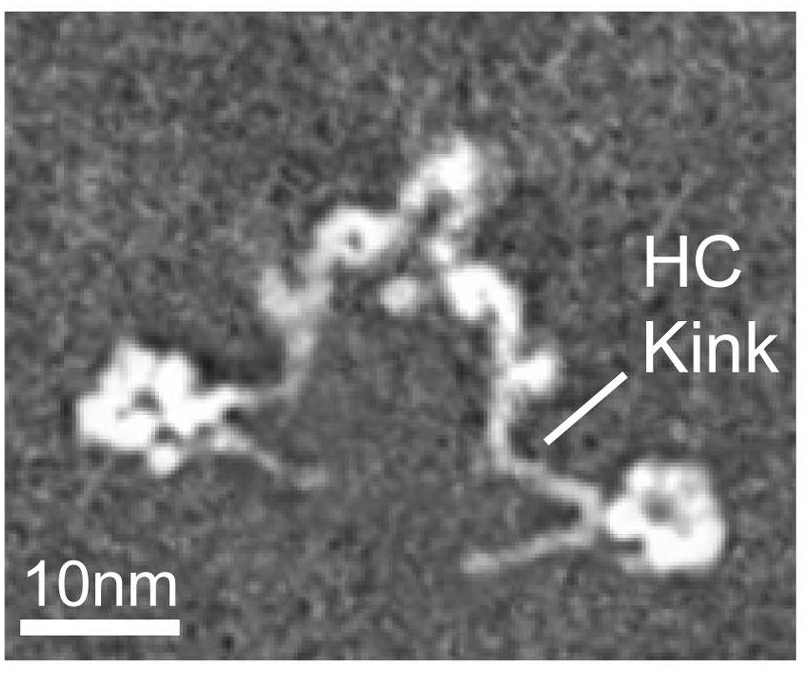
\includegraphics[width=0.3\columnwidth]{figures/schematic-1-cryoem}
%%    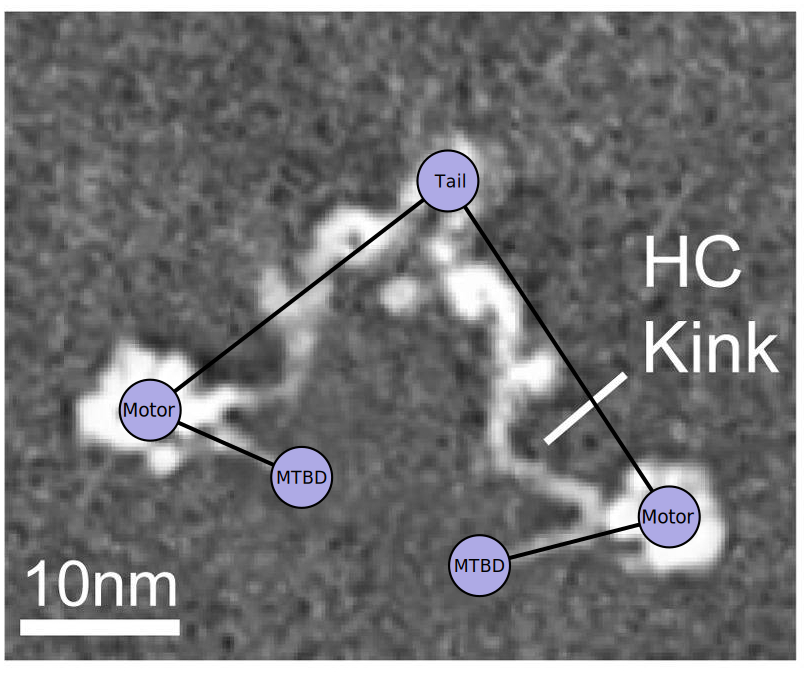
\includegraphics[width=0.3\columnwidth]{figures/schematic-1-superimposed}
%%    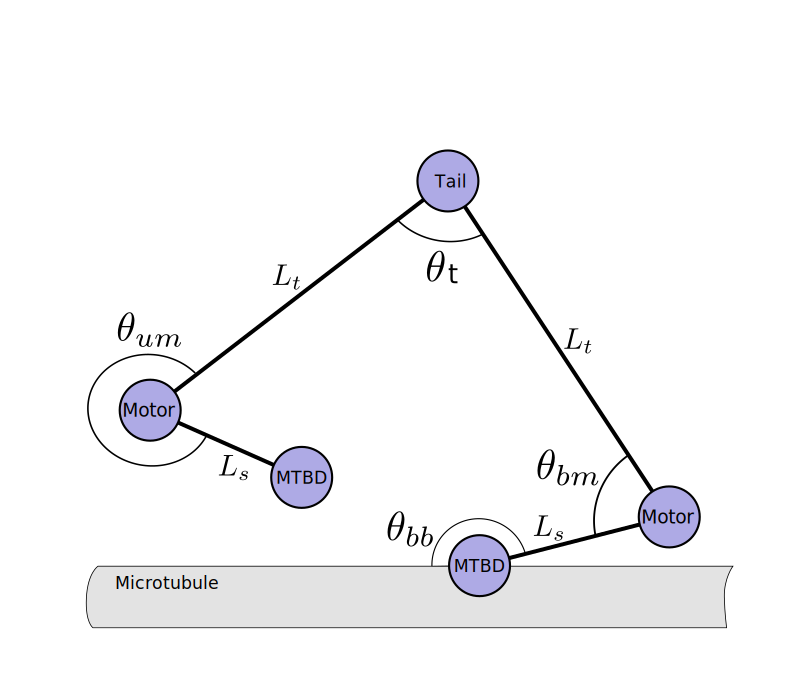
\includegraphics[width=0.3\columnwidth]{figures/schematic-1-model}

%%    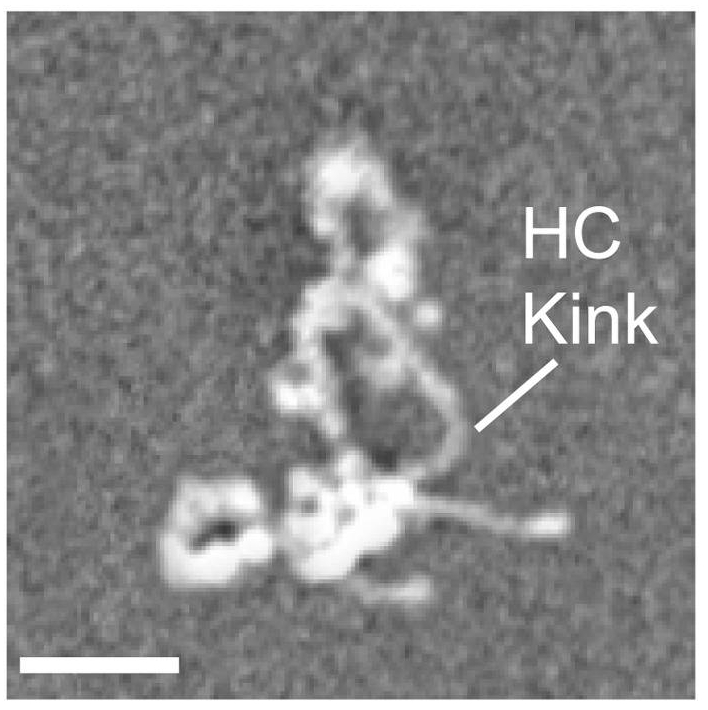
\includegraphics[width=0.3\columnwidth]{figures/schematic-2-cryoem}
%%    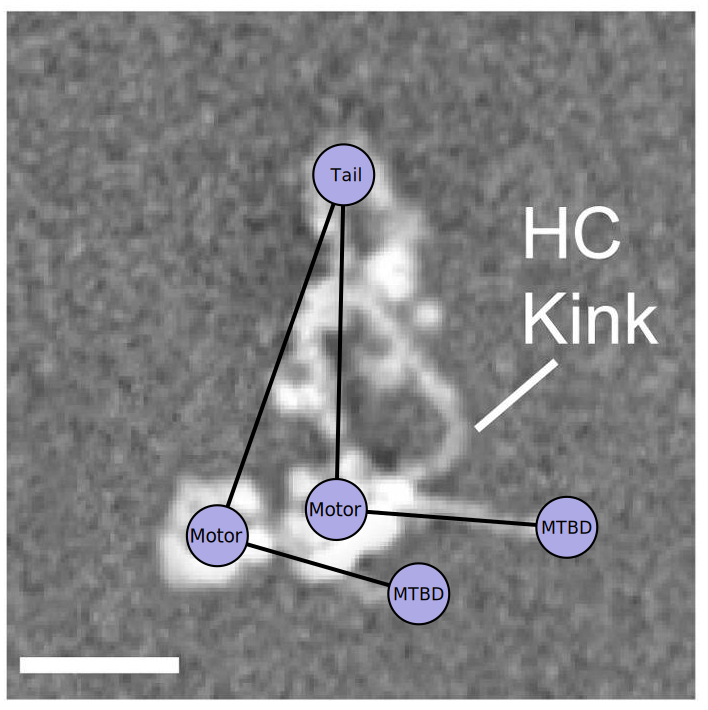
\includegraphics[width=0.3\columnwidth]{figures/schematic-2-superimposed}
%%    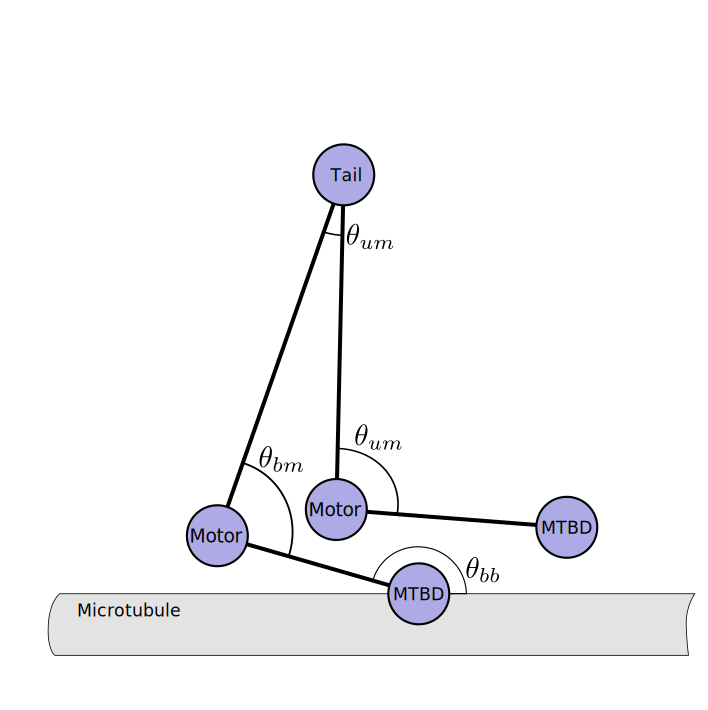
\includegraphics[width=0.3\columnwidth]{figures/schematic-2-model}
%%    \caption{\textbf{Model schematic superimposed on cryo-EM images of
%%        native dynein.} Native cryo-EM images of the full dimerized
%%      dynein complex composed of light, intermediate and heavy chains,
%%      from \cite{nativestructure}. Model schematics are superimposed
%%      for illustrative purpose; shown angles to not represent expected
%%      \textit{in vivo} equilibria. Schematics are shown docked to a
%%      microtubule for illustrative purposes.}
%%    \label{fig:modelparams}
%% \end{figure}

%% \begin{figure}[tbhp]
%%   \centering
%% 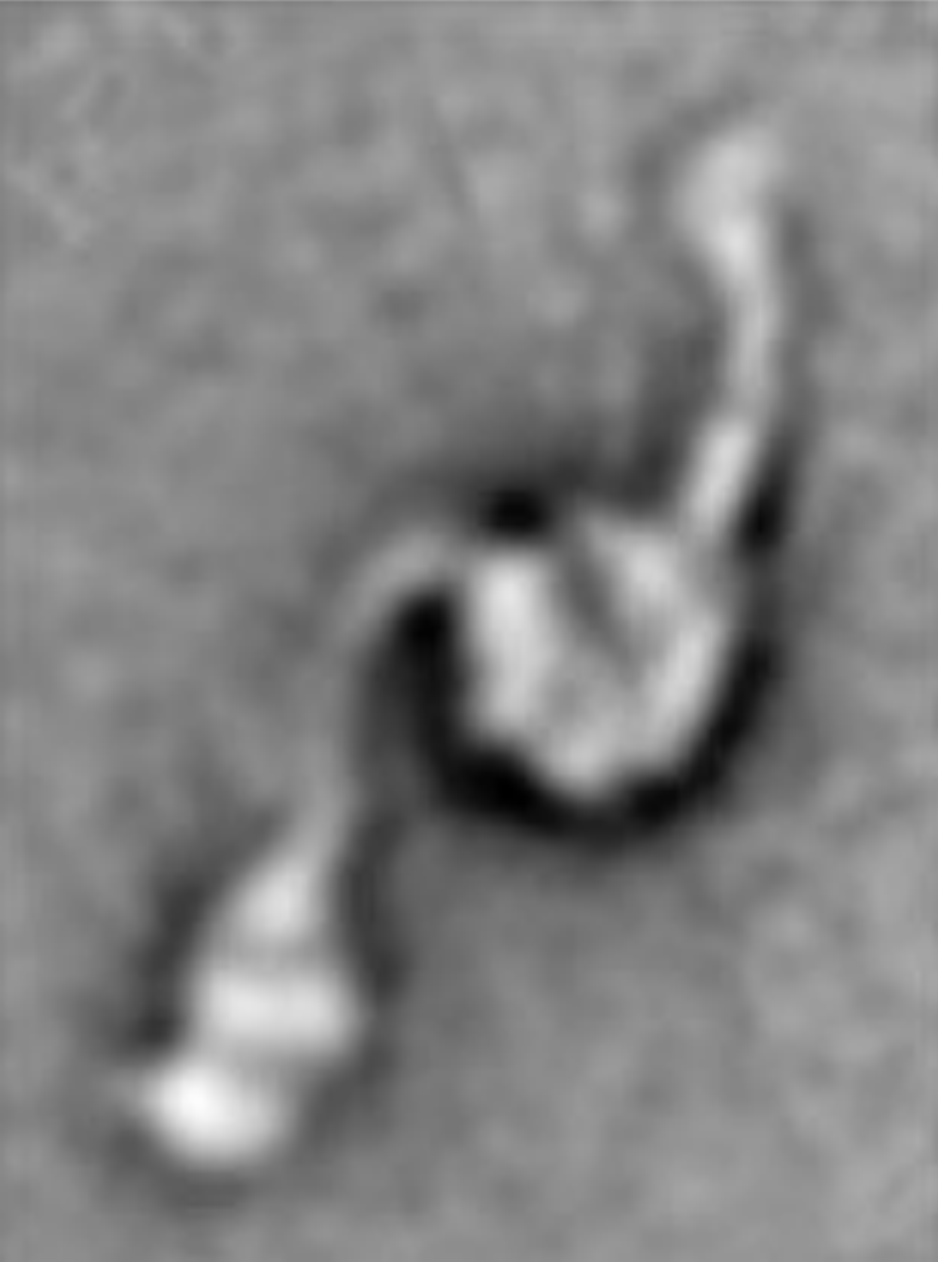
\includegraphics[width=0.5\columnwidth]{figures/schematic-prestroke}%
%% \includegraphics[width=0.5\columnwidth]{figures/schematic-poststroke}\\
%% \includegraphics[width=0.5\columnwidth]{figures/schematic-binding-angle}%
%% \includegraphics[width=0.5\columnwidth]{figures/schematic-full}
%%   \caption{\textbf{Schematic of model equilibrium angles over cryo-EM
%%       images.} \textbf{a.)} Prestroke and \textbf{b.)} poststroke
%%     dynein heavy chains superimposed with model motor angles, both
%%     from \cite{burgess-paper}. \textbf{c.)} Axonemal dynein bound to
%%     MT with model binding angle superimposed, from
%%     \cite{leschziner}. \textbf{d.} Full native dynein cryo-EM image
%%     bound to an MT with model superimposed, from
%%     \textbf{nativestructure}.}
%% \label{fig:modelangles}
%% \end{figure}

\showmatmethods

\section{To do items}

\subsection{Elliott}
\begin{enumerate}
\item Fix stepping analysis python module to categorize zero-length
  steps separately from other steps, particularly in terms of stepping
  times.  Alternately, change C++ to make it possible to identify
  which foot lifted if it didn't move.
\item When we have all data, write discussion
\item Rewrite introduction
\item Possibly sample stalk angles at high resolution and also 50ms, to show why the low time resolution in Lessinger prevented them from seeing the powerstroke?
\item Test suite for paper plots to see if there aren't subtle bugs?
\item Re-run velocity vs force simulation at a much lower rate to match the Gennerich velocity at pN=0
\end{enumerate}

\subsection{John}
\begin{enumerate}
\item Proofread the algorithm description, improve its writing, and
  check against code.
\item Run a low-ATP simulation for comparison data.
\item Consider a no-binding simulation and a separable model.  Create
  a figure demonstrating/testing whether the histogram of final
  displacement is independent of initial displacement.
\item Consider a simple Monte Carlo that just uses our no-unbinding
  and no-binding simulations to model dynein (like Yildiz).
\end{enumerate}

\section{Papers we should cite}
This paper says something interesting~\cite{leschziner}.

% \pnasbreak splits and balances the columns before the references.
% If you see unexpected formatting errors, try commenting out this line
% as it can run into problems with floats and footnotes on the final page.
\pnasbreak

\bibliography{paper}

\end{document}
